\documentclass[12pt]{article}
\usepackage[utf8]{inputenc}
\usepackage[french]{babel}
\usepackage{amsmath,amssymb}
\usepackage{graphicx}
\usepackage{geometry}
\usepackage{caption}
\geometry{a4paper, margin=2.5cm}
\usepackage{float}

\title{Leçon 13 : Transformations du plan.\\ Frises et pavages}
\author{}
\date{}

\begin{document}

    \maketitle

    \section*{Prérequis}
    \begin{itemize}
        \item Médiatrice
        \item Angle et longueur
        \item Polygones et polygones réguliers
    \end{itemize}
    \textit{Niveau : Collège (Cycle 4), Première, Terminale STD2A}

    \tableofcontents
    \newpage

    \section{Transformations du plan}

    \subsection{Introduction}
    Une transformation \( t \) associe à une figure \( F \) du plan une autre figure \( F' \) du plan. On dit que \( F' \) est l'image de \( F \) par la transformation \( t \), et \( F' \) est unique.

    \[
        t : F \rightarrow t(F) = F'
    \]

%SYMETRIE AXIALE =========================================
    \subsection{Symétrie axiale}

    \textbf{Définition :} Le symétrique d’un point \( A \) par rapport à une droite \( (D) \) est le point \( M \) tel que \( (D) \) soit la médiatrice du segment \( [AM] \).

    Deux figures sont symétriques par rapport à une droite si elles se superposent par pliage le long de cette droite. Cette droite est appelée l’axe de symétrie.

    \begin{figure}[h!]
        \centering
        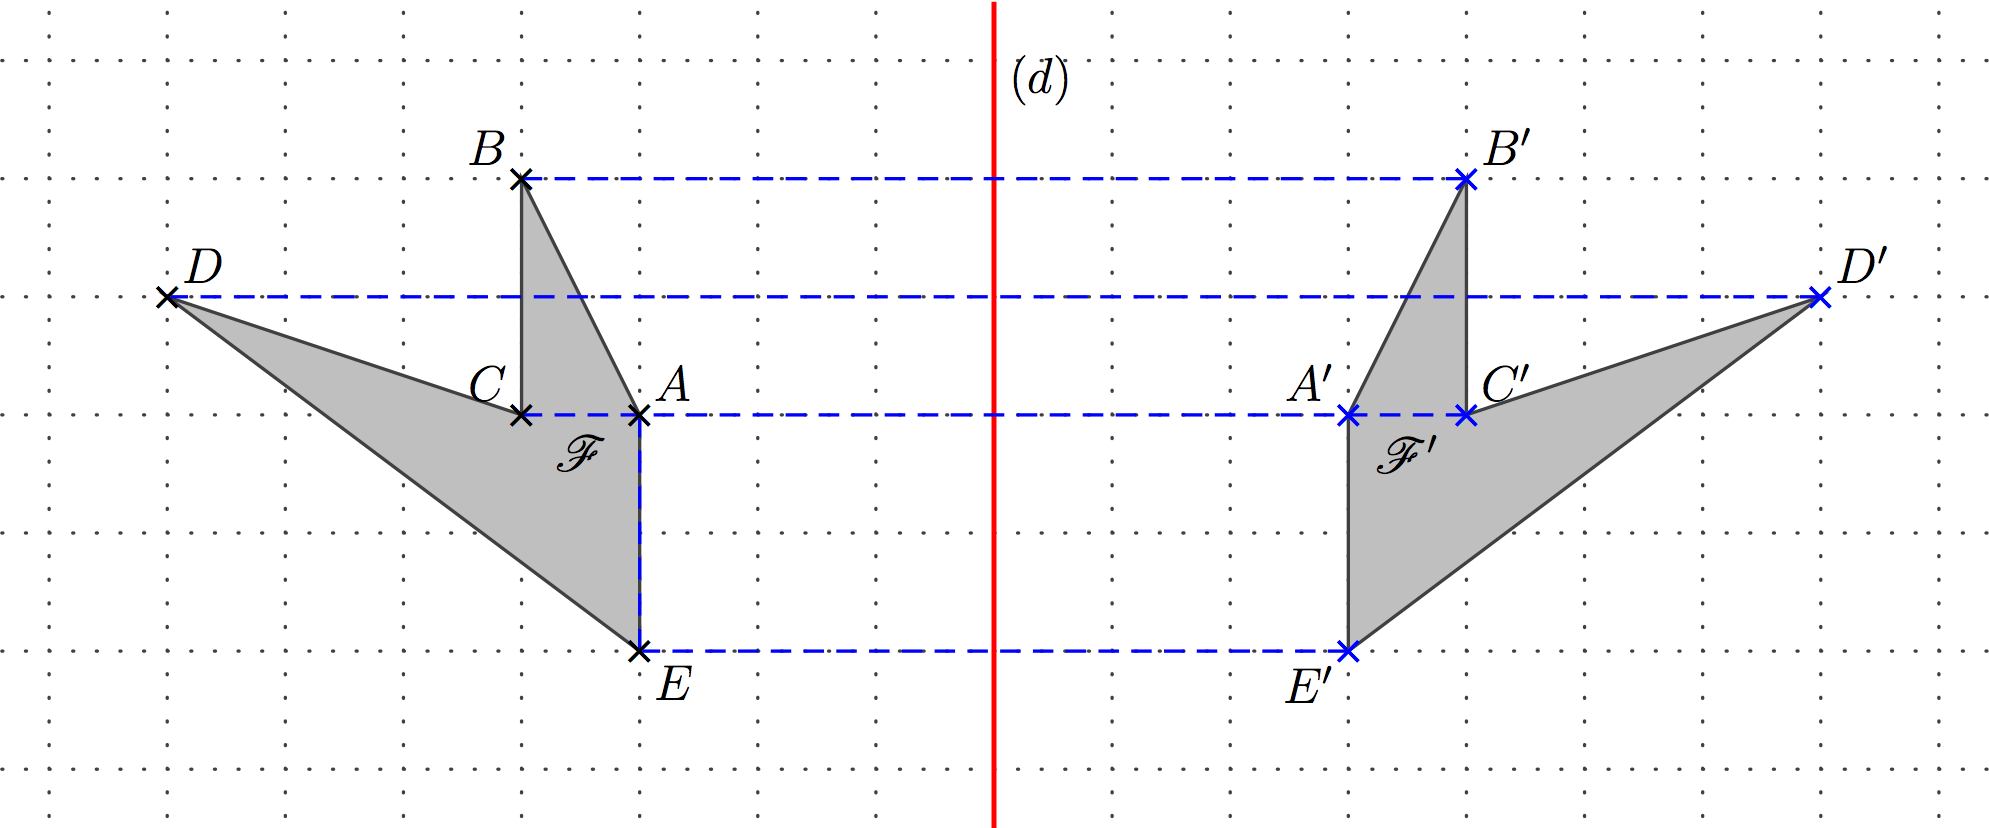
\includegraphics[width=0.5\textwidth]{symetrie_axiale.png}
        \caption{Illustration de la symétrie axiale}
    \end{figure}

    %ROTATIONS =========================================
    \subsection{Rotation}

    \textbf{Définition :} La rotation de centre \( O \), d’angle \( \alpha \), dans un sens donné, du point \( M \) du plan est le point \( M' \) tel que le triangle \( OMM' \) soit isocèle en \( O \) et que l’angle \( \widehat{(OM, OM')} = \alpha \).

    \begin{figure}[H]
        \centering
        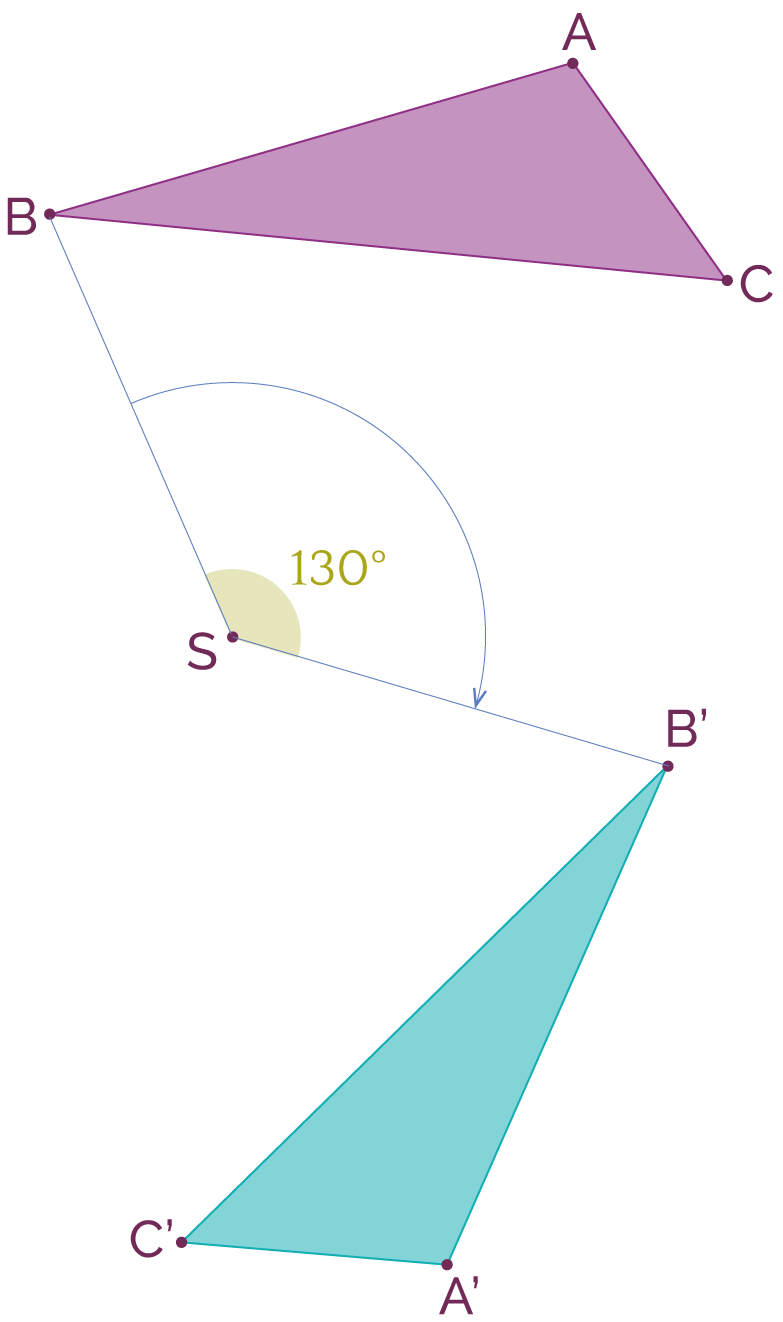
\includegraphics[width=0.5\textwidth]{rotation.png}
        \caption{Exemple de rotation de centre \( O \), angle 130° (sens horaire)}
    \end{figure}
%SYMETRIE CENTRALE =========================================
    \subsection{Symétrie centrale}

    \textbf{Définition :} Soit un point \( M \) du plan. Son image \( M' \) par une symétrie centrale de centre \( O \) est tel que \( O \) est le milieu de \( [MM'] \).

    \textbf{Remarque :} Une symétrie centrale équivaut à une rotation d’angle 180° autour du centre de symétrie.

    %TRANSLATION =========================================
    \subsection{Translation}

    \textbf{Définition :} Soient deux points \( A \) et \( B \). La translation qui envoie \( A \) sur \( B \) à un point \( M \) est le point \( M' \) obtenu en glissant selon la direction de \( (AB) \), dans le sens de \( A \) vers \( B \), et de longueur \( AB \).

    \textbf{Notation :} Représentée par une flèche \( \vec{AB} \).
    \begin{figure}[H]
        \centering
        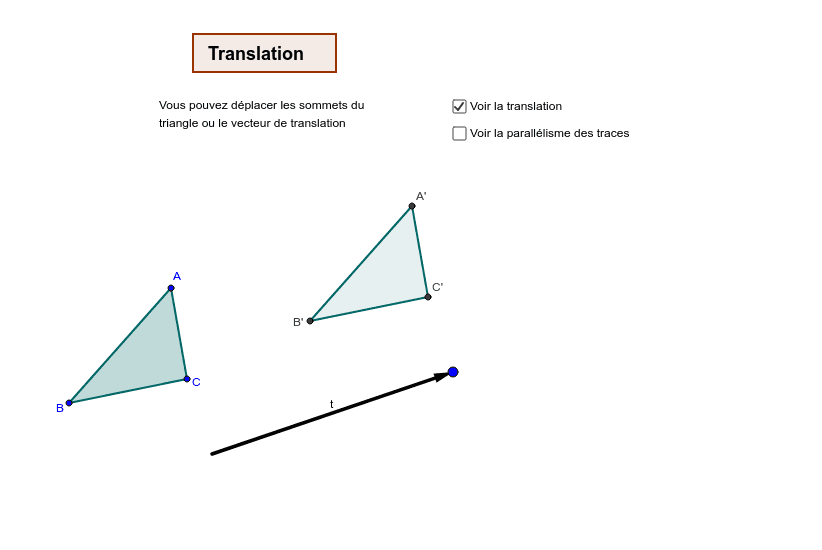
\includegraphics[width=0.5\textwidth]{translation.png}
        \caption{Exemple de translation}
    \end{figure}
    \subsection{Propriétés}

    \begin{itemize}
        \item Les transformations conservent l’alignement, les distances, les angles, les aires, le parallélisme et l’orthogonalité.
        \item Une symétrie axiale, centrale ou une translation transforme une droite en une droite parallèle.
    \end{itemize}

    %FRISES ===============================================
    \section{Frises}

    \subsection{Définitions}

    \textbf{Bande (ou ruban) :} Portion du plan comprise entre deux droites parallèles.

    \textbf{Frise :} Une frise est un motif répété indéfiniment par translation le long d'une direction (en général parallèle aux deux droites délimitant la bande). On parle de \textit{frise périodique}.

    \textbf{Motif élémentaire :} Plus petite figure permettant de reconstituer toute la frise par application d’isométries.

    \textbf{Motif de base :} Motif complet avant répétition par translation. Il peut être obtenu à partir du motif élémentaire par d'autres transformations (symétries, rotations...).

    \begin{figure}[h!]
        \centering
        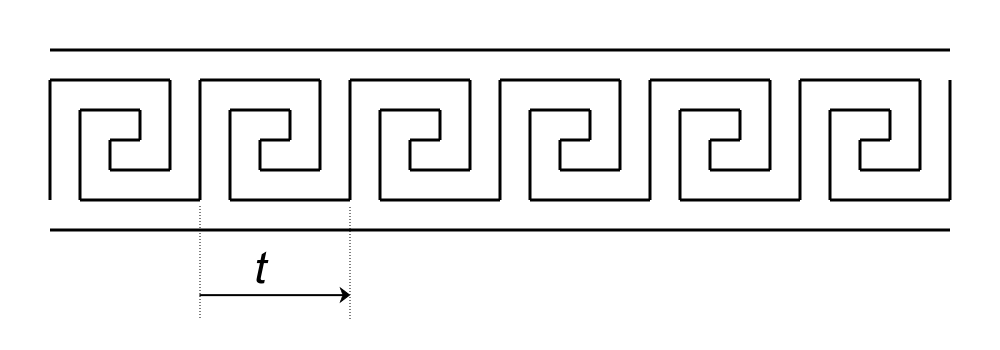
\includegraphics[width=\textwidth]{frise_exemple.png}
        \caption{Exemple de pavage avec un lutin}
    \end{figure}

    \subsection{Les isométries du plan dans les frises}

    Outre la translation, une frise peut présenter d’autres symétries :

    \begin{itemize}
        \item Symétrie axiale horizontale (par rapport à l’axe médian de la bande)
        \item Symétrie axiale verticale (perpendiculaire à la direction de la frise)
        \item Symétrie centrale
        \item rotation de 180°
    \end{itemize}


    \subsection{Activité possible - Exploration avec GeoGebra}

    \textbf{Objectif :} Explorer la diversité des frises en créant un motif et en lui appliquant diverses isométries.
    \begin{figure}[h!]
        \centering
        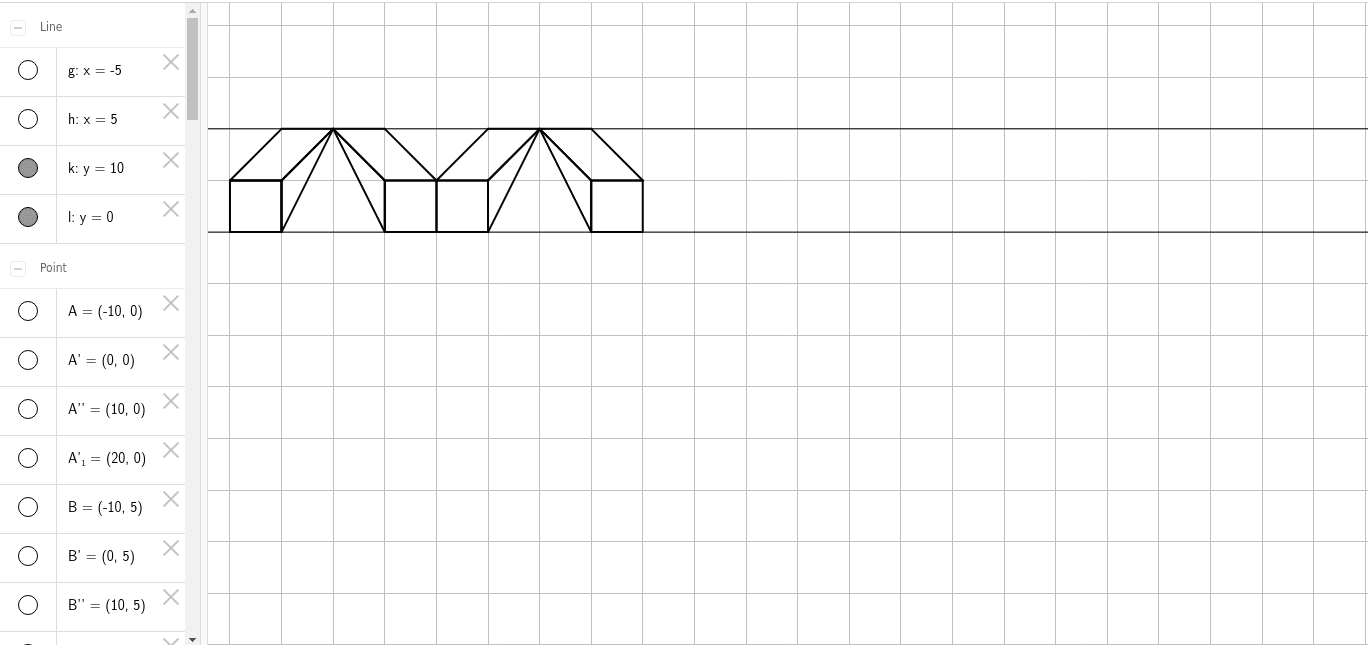
\includegraphics[width=\textwidth]{geogebra_frise.png}
        \caption{Exemple de frise créée avec GeoGebra}
    \end{figure}
    \begin{enumerate}
        \item Créer un motif élémentaire.
        \item Répéter ce motif par translation.
        \item Ajouter selon les cas : une symétrie axiale verticale, une symétrie horizontale, une rotation d’ordre 2.
    \end{enumerate}



%PAVAGES ========================================
    \section{Pavages}

    \subsection{Définitions et propriétés}

    \textbf{Définition :} Un pavage est une portion du plan où un motif de base se répète régulièrement par deux translations non parallèles (ex. \( A \rightarrow B \) et \( A \rightarrow C \)).

    \textbf{Proposition :} Les seuls pavages réguliers du plan sont par :
    \begin{itemize}
        \item triangles équilatéraux
        \item carrés
        \item hexagones réguliers
    \end{itemize}

    \textbf{Propriété :} Soit \( ABCD \) un parallélogramme. En appliquant des translations de \( D \rightarrow A \) et \( D \rightarrow C \), on obtient un pavage.

    \subsection{Application - Activité Scratch}

    \textbf{Consigne :} Programmer un pavage du plan en répétant un motif comme le lutin « stop ».

    \begin{figure}[h!]
        \centering
        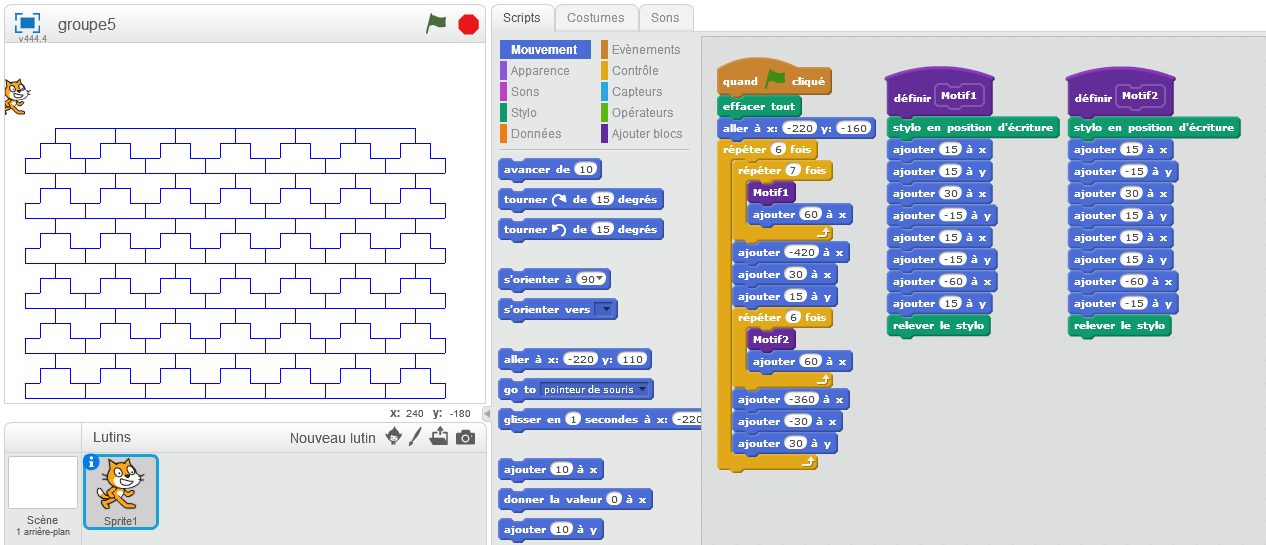
\includegraphics[width=1.2\textwidth]{scratch_pavage.png}
        \caption{Exemple de pavage avec un lutin}
    \end{figure}

\end{document}
